%Springer Nature LaTeX template, version 3.1 (December 2024)
\documentclass[pdflatex,referee]{sn-jnl}% referee: double line spacing
% Vancouver numbered references as with the class option sn-vancouver-num, but using
% bmc-vancouver.bst, which prints web references in BMC form (URL, then "Accessed date").
\usepackage[numbers,sort&compress]{natbib}%
\gdef\NumBib{YES}%
\bibliographystyle{bmc-vancouver}%
\setlength{\bibsep}{1em}%
\makeatletter\def\bibfont{\reset@font\fontfamily{\rmdefault}\normalsize\selectfont}\makeatother%
\usepackage{graphicx}%
\graphicspath{{figures/}}%
\usepackage{multirow}%
\usepackage{amsmath,amssymb,amsfonts}%
\usepackage{textcomp}%
\usepackage{manyfoot}%
\usepackage{booktabs}%
\usepackage{array}%
\usepackage{xurl}%
\usepackage[mathlines]{lineno}%
\linenumbers
\raggedbottom

\begin{document}

\title[Laboratory relationships in synthetic clinical tables]{Evaluating and preserving laboratory relationships in synthetic clinical tables}

\author[1]{\fnm{Naren} \sur{Medarametla}}\email{naren.medarametla2023@vitstudent.ac.in}
\author[1]{\fnm{Abishek} \sur{K G}}\email{abishek.kg2023@vitstudent.ac.in}
\author[1]{\fnm{Roshan} \sur{Parveen}}\email{roshan.parveen2023@vitstudent.ac.in}
\author*[1]{\fnm{Parkavi} \sur{K}}\email{parkavi.k@vit.ac.in}

\affil[1]{\orgdiv{School of Computer Science and Engineering}, \orgname{Vellore Institute of Technology, Chennai Campus}, \orgaddress{\street{Vandalur-Kelambakkam Road}, \city{Chennai}, \postcode{600127}, \state{Tamil Nadu}, \country{India}}}

\abstract{\textbf{Background:} Synthetic clinical tables are judged by empirical evaluation, yet laboratory data are small, reported on fixed grids and linked by formulas that hold exactly or only up to rounding. We studied how to evaluate such tables and preserve their laboratory relationships.

\textbf{Methods:} In a prospectively specified study on two public populations, a National Health and Nutrition Examination Survey (NHANES) biochemistry cohort and a thyroid registry, we compared twelve generator variants under uncorrected and corrected training and evaluation pipelines and decomposed the training correction. We then formalized relation reparameterization, which replaces one participant of each supplied relation by a learned residual, and tested it in a hypergraph-guided diffusion model on five NHANES datasets from four survey cycles, against five published generators and post-processing controls with the same knowledge of the relations. Realism, utility and memorization were measured by classifier two-sample tests, by training on synthetic and testing on real records, and by two membership attacks, with one membership threshold of 0.60 for every method.

\textbf{Results:} Correcting the pipeline reversed 25\% to 34\% of generator pairs and changed the top-ranked generator in 18 of 20 training samples; a decomposition traced the training effect to an epoch cap that left small tables undertrained, not to validation-based checkpoint selection. Formulas computed exactly from reported values were reproduced best by recomputing them. Approximate blood count formulas needed their residuals kept and sampled jointly: recomputation over-corrected them and independent residual noise broke their coupling, whereas joint resampling of real residuals and learned residual coding preserved it. The learned model reproduced the approximate relations most closely in every setting, by a small margin over the best control, and was the most realistic generator below the membership threshold in five of ten settings, all at 250 or 1000 records; TabDiff or simple controls were as realistic or more elsewhere.

\textbf{Conclusions:} Routine training and evaluation choices can determine which synthetic data generator appears best on small clinical tables. Laboratory formulas computed exactly should be recomputed, whereas approximate ones need jointly sampled residuals. Membership diagnostics are not privacy guarantees, and the contribution of the hypergraph was not isolated.}

\keywords{Synthetic data, Tabular data, Diffusion models, Laboratory data, Electronic health records, Evaluation methodology, Membership inference, NHANES}

\maketitle

\section*{Background}

Synthetic data are increasingly proposed as a way to share clinical tables without exposing patients. Whether a synthetic table is faithful, useful and safe is decided almost entirely by empirical evaluation: classifier two-sample tests, distances between marginal and joint distributions, models trained on synthetic data and tested on real data, checks of clinical rules, and distance-based or attack-based privacy diagnostics. Clinical tables are typically small, their laboratory values are heavy-tailed and reported on fixed grids, some measurements are missing, and several variables are linked by formulas. Some formulas hold exactly at the reported precision, such as a globulin value computed from reported total protein and albumin; others hold only approximately, such as red cell indices that an analyzer computes from unrounded internal measurements. These properties interact with ordinary training and evaluation choices in ways that are easy to overlook.

This work began as the development of a constraint-guided diffusion model for medical tables. Ten development iterations produced mixed, partition-dependent conclusions, and an audit showed that most of them were produced by training and evaluation choices rather than by the models. We describe seven such pitfalls and quantify them in a controlled study. We then use the corrected protocol to develop and test a generator that reproduces laboratory relationships, and we report where it is better than published generators and simple controls and where it is not.

\subsection*{Tabular data generators}

Tabular data generators range from statistical copulas to generative adversarial networks and variational autoencoders, of which CTGAN and TVAE are the standard references \cite{xu2019ctgan}. Diffusion models \cite{ho2020ddpm,austin2021d3pm} were adapted to mixed tables by TabDDPM \cite{kotelnikov2023tabddpm}, which combines Gaussian and multinomial diffusion, and by TabDiff \cite{shi2025tabdiff}, which uses continuous-time diffusion with learnable per-column noise schedules. Feature relationships have been modeled with learned graphs in GOGGLE \cite{liu2023goggle}. For longitudinal patient records, Momenzadeh and Oshaghi combined a deep encoder-decoder with a hidden Markov layer and evaluated statistical similarity, temporal consistency, compliance with clinical rules, privacy and downstream accuracy \cite{momenzadeh2026dghmm}. There, clinical rules are one dimension on which the generated data are scored; MedHyperDiff instead builds the supplied laboratory relations into the representation that the generator learns.

\subsection*{Dependency-aware and constraint-aware generation}

Umesh \textit{et al.} showed that common generators do not preserve functional dependencies between attributes \cite{umesh2024dependencies}, and their hierarchical feature generation framework generates independent features with an existing generator and reconstructs dependent features deterministically from supplied dependency rules \cite{umesh2025hfgf}. That framework targets mainly categorical dependencies and sets dependent values exactly by the rule. Our method differs in three respects: it models the discrepancy of each numerical relation as a learned residual instead of assuming exactness, it chooses which participant to reconstruct from the data to limit error propagation, and it accounts for the recording resolution of reported values. Constraint-aware generation also includes the constraint layers of C-DGM \cite{stoian2024cdgm} and DRL \cite{stoian2025drl} and the inference-time manifold guidance of Harpoon \cite{shankar2026harpoon}. We did not run these methods. Our deterministic re-derivation controls enforce the supplied relations exactly after generation and should not be read as reimplementations of them.

\subsection*{Evaluation of synthetic data}

Evaluation commonly combines classifier two-sample tests \cite{lopezpaz2017c2st}, marginal and dependence distances, downstream utility and privacy diagnostics such as distance to the closest record, membership inference by overfitting detection \cite{vanbreugel2023domias} and attack-based audits \cite{giomi2023anonymeter}. Integrated frameworks combine these dimensions: Kim \textit{et al.} jointly assessed distributional fidelity, privacy risk and diagnostic utility of VAE and CTGAN data from a severely imbalanced cohort, stratifying every metric by disease prevalence, and showed that single-metric evaluation misses failure modes in minority classes \cite{kim2026integrated}. The difficulty of estimating uncertainty from overlapping resamples is well known \cite{bengio2004variance}. We do not propose a new metric family or framework. Our evaluation question is complementary: holding the metrics fixed, we show how ordinary training and evaluation choices, such as the training budget, the scaling of heavy-tailed values, the scoring of clinical rules and the size of the evaluation set, change which generator appears best on small clinical tables, and we add relation fidelity, measured against the recording resolution of each variable, as a dimension that existing frameworks do not assess.

\subsection*{Aims}

This study has three aims. First, we catalogue seven training and evaluation pitfalls, quantify how much they change the ranking of generators on two public populations, and decompose the training correction into its components. Second, we formalize relation reparameterization with learned residuals, a conditioning-based reconstruction direction and re-derivation of exactly reported values, and we position it against rule-based reconstruction of dependent features. Third, on five NHANES panel-by-cycle datasets we compare it with five published generators and with post-processing controls that use the same knowledge of the relations, including textbook re-derivation and joint resampling of real residuals, and we identify which treatment each kind of relation needs and where a learned model adds to simple controls.

\section*{Methods}

\subsection*{Overview}

MedHyperDiff is a mixed-type diffusion model with Gaussian diffusion for numerical values, absorbing-mask diffusion for categories and explicit missingness indicators (Fig.~\ref{fig:pipeline}). Its denoiser is a feature transformer with an attention bias from a bootstrap-stable association graph and nonlinear hyperedge message passing over supplied clinical relations. Relation reparameterization, described below, replaces one participant of each supplied laboratory relation by a residual before diffusion and rebuilds it after decoding. The source code, study protocols and the results underlying every table and figure are available online \cite{code}. The study has five parts: a development case study that exposed the pitfalls, a controlled study that quantifies them, an experiment that decomposes the training correction, a first relation test on blood counts, and a robustness study across survey cycles, relation types and sample sizes.

\begin{figure}[htbp]
\centering
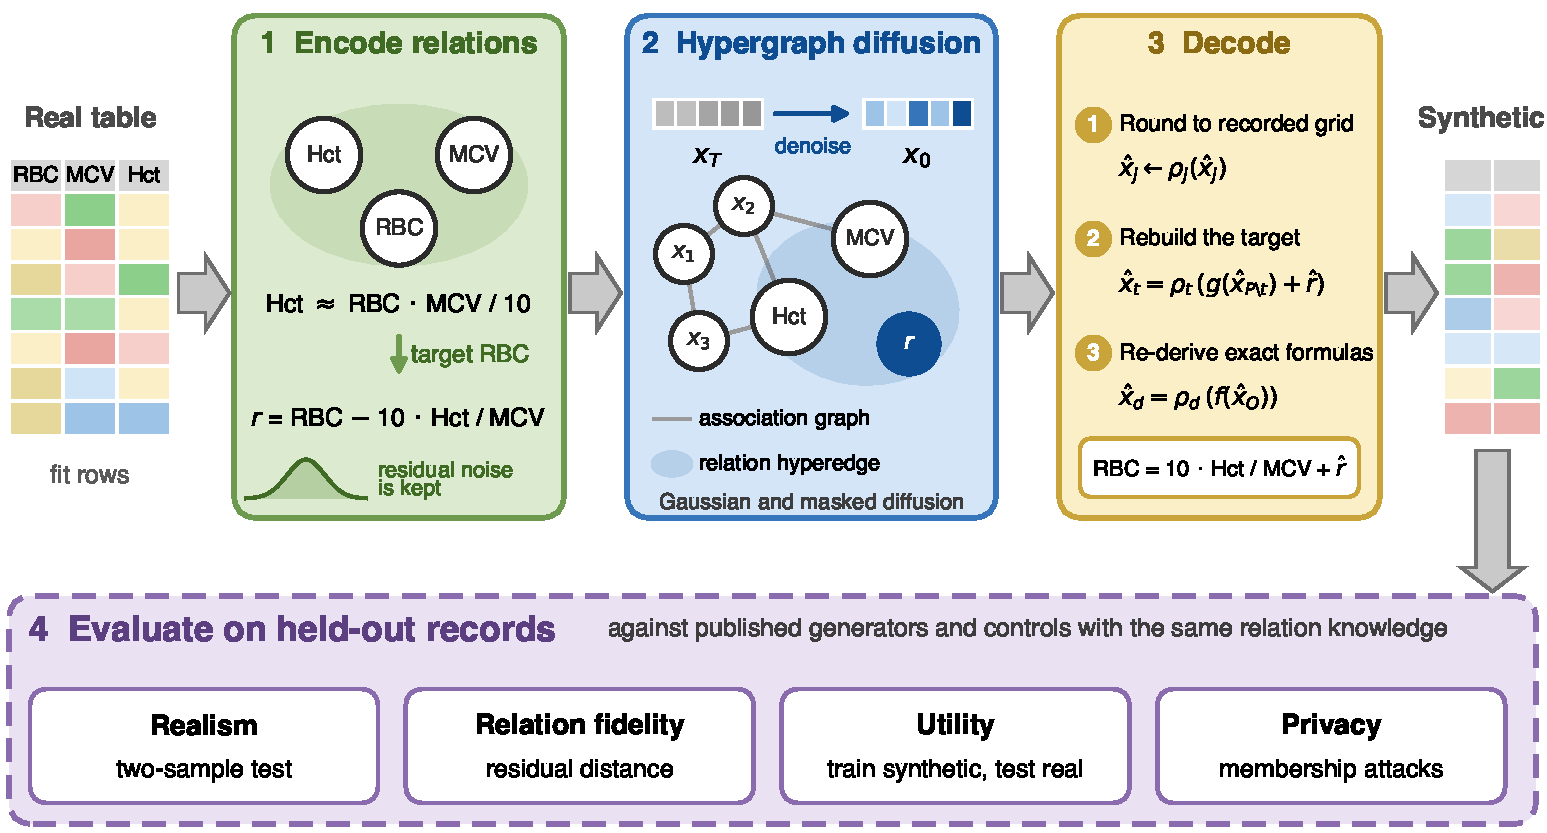
\includegraphics[width=\textwidth]{Figure1.pdf}
\caption{\textbf{Overview of MedHyperDiff.} (1) One participant of each supplied laboratory relation is replaced by a residual $r$, shown for hematocrit (Hct), red blood cell count (RBC) and mean corpuscular volume (MCV). (2) A diffusion model generates the remaining variables and the residuals; its denoiser uses an association graph as attention bias and one hyperedge per relation. (3) Generated values are rounded to the recorded resolution $\rho$, the replaced participant is rebuilt from its residual, and relations that laboratories compute exactly are re-derived. (4) Synthetic tables are evaluated on held-out records against published generators and post-processing controls that use the same knowledge of the relations.}
\label{fig:pipeline}
\end{figure}

\subsection*{Datasets}

All datasets are public and de-identified (Table~\ref{tab:data}). The development case study used four cohorts from the University of California, Irvine (UCI) Machine Learning Repository: the Indian Liver Patient Dataset \cite{ilpd}, heart failure clinical records \cite{heartfailure,chicco2020}, chronic kidney disease \cite{ckd} and early-stage diabetes risk prediction \cite{diabetes}. The controlled study used adults in the National Health and Nutrition Examination Survey (NHANES) 2017 to 2018 \cite{nhanes2017} with a standard biochemistry record (21 numerical predictors and sex; label: diagnosed diabetes) and the UCI thyroid registry \cite{thyroid} (six numerical and sixteen categorical predictors, up to 28\% missing; label: any thyroid diagnosis).

The relation studies used NHANES complete blood count and chemistry panels from four survey cycles \cite{nhanes2011,nhanes2013,nhanes2017,nhanes2021}. In the blood count panel the analyzer measures red cell count, hemoglobin and mean corpuscular volume and computes hematocrit, mean corpuscular hemoglobin and mean corpuscular hemoglobin concentration from unrounded internal values, so these relations, and the sum of the five white cell differential percentages, hold only up to rounding. In the chemistry panel NHANES computes all four relations from reported values, and an audit before fitting found each of them exact at reported precision. NHANES samples different people in each cycle, but datasets from the same cycle share participants, so the blood count results come from three survey cycles and the chemistry results from two. Two further datasets from 2015 to 2016 \cite{nhanes2015} were used only to choose the training budget.

\begin{table}[htbp]
\caption{Datasets of the controlled study and the relation studies}
\label{tab:data}
\footnotesize
\begin{tabular}{@{}>{\raggedright\arraybackslash}p{0.15\textwidth}>{\raggedright\arraybackslash}p{0.36\textwidth}r>{\raggedright\arraybackslash}p{0.31\textwidth}@{}}
\toprule
Study & Dataset & Records & Supplied relations \\
\midrule
Controlled & NHANES 2017 to 2018 biochemistry & 4756 & Globulin and BMI (exact) \\
Controlled & UCI thyroid registry & 9172 & Free thyroxine index (approximate) \\
First relation test & NHANES 2017 to 2018 blood count & 4865 & Hct, MCH, MCHC and white cell differential (approximate) \\
Robustness & NHANES 2013 to 2014 blood count & 5229 & As above (approximate) \\
Robustness & NHANES 2021 to 2023 blood count & 5555 & As above (approximate) \\
Robustness & NHANES 2011 to 2012 chemistry & 4778 & Globulin, BMI, ACR and osmolality (exact) \\
Robustness & NHANES 2021 to 2023 chemistry & 5284 & As above (exact) \\
\botrule
\end{tabular}
\footnotetext{Relations: globulin = total protein $-$ albumin; BMI = weight/height$^2$; free thyroxine index = total thyroxine/thyroid hormone uptake; Hct = RBC $\times$ MCV/10; MCH = 10 $\times$ hemoglobin/RBC; MCHC = 100 $\times$ hemoglobin/Hct; the five white cell differential percentages sum to 100; ACR = 100 $\times$ urine albumin/urine creatinine; osmolality = 1.86 Na + glucose/18 + BUN/2.8 + 9, with sodium in mmol/L and glucose and BUN in mg/dL. Exact: the relation holds at reported precision. ACR, urine albumin to creatinine ratio; BMI, body mass index; BUN, blood urea nitrogen; Hct, hematocrit; MCH, mean corpuscular hemoglobin; MCHC, mean corpuscular hemoglobin concentration; MCV, mean corpuscular volume; RBC, red blood cell count.}
\end{table}

\subsection*{Relation reparameterization}

A supplied relation $k$ links a derived variable $x_{d_k}$ to operands $x_{O_k}$ through a known function, $x_{d_k} = f_k(x_{O_k}) + \varepsilon_k$, where $\varepsilon_k$ collects rounding and analyzer effects and is zero only for relations computed exactly. Every participant $j \in P_k = \{d_k\} \cup O_k$ can be solved for, $x_j = g_{kj}(x_{P_k \setminus j}) + \varepsilon_{kj}$. Relation reparameterization chooses one target $t_k \in P_k$ per relation and replaces $x_{t_k}$ by the residual
\begin{equation}
r_k = x_{t_k} - g_{k t_k}\!\left(x_{P_k \setminus t_k}\right).
\label{eq:residual}
\end{equation}
The generator models the joint distribution of the remaining variables and the residuals, so rounding noise and rare discrepancies are learned rather than forced to zero or ignored. After sampling, every generated variable is decoded to its recording resolution $\rho_j$, detected on fit rows, and the targets are reconstructed in an acyclic order,
\begin{equation}
\hat{x}_{t_k} = \rho_{t_k}\!\left( g_{k t_k}(\hat{x}_{P_k \setminus t_k}) + \hat{r}_k \right).
\label{eq:decode}
\end{equation}
A relation is treated as reported exactly when at least 99\% of complete fit rows satisfy $|x_{d_k} - f_k(x_{O_k})| \le \delta_{d_k}/2$, where $\delta_{d_k}$ is the recording step of the derived variable. For such relations the decoder finally sets $\hat{x}_{d_k} = \rho_{d_k}(f_k(\hat{x}_{O_k}))$, the computation the laboratory performs, so that rounding a reconstructed operand does not create discrepancies that real records do not have.

\subsection*{Choosing the reconstructed participant}

Errors in the generated participants propagate into the reconstructed one. On the scale on which relation $k$ is additive, $\sum_{j \in P_k} a_{kj}\, \phi_k(x_j) = c_k$, with $\phi_k$ the logarithm for products and ratios and the identity for sums, differences and linear formulas, a generation error $e_j$ in participant $j$ moves the reconstructed target $t$ by approximately $-a_{kt}^{-1} \sum_{j \ne t} a_{kj} e_j$. Relative to the spread of the target, $s_{kt} = |a_{kt}|\, \mathrm{sd}(\phi_k(x_t))$, this error is smallest for the participant with the largest $s_{kt}$ when generated participants have comparable errors. For body mass index, which is additive on the logarithmic scale as $\log \mathrm{BMI} = \log w - 2\log h + c$, height therefore enters with coefficient 2. We therefore choose
\begin{equation}
(t_1, \dots, t_K) = \arg\max \textstyle\sum_{k} s_{k t_k}
\label{eq:choice}
\end{equation}
over assignments with distinct targets that admit an acyclic reconstruction order, estimating $s$ on fit rows only. The rule rests on this first-order argument and is a heuristic, not a guarantee of optimal conditioning. It enumerates $\prod_k |P_k|$ assignments, 135 for the four blood count relations used below, which is small for a laboratory panel but grows exponentially with the number of relations.

\subsection*{Model and training}

In MedHyperDiff each residual and the participants it depends on, expanded recursively through earlier reconstructions, form a hyperedge of the denoiser. The model is trained with a velocity-prediction loss on observed numerical values, an absorbing-state cross-entropy for categories and observation indicators, and a small physical-range energy, with linear learning-rate decay and weight averaging. The number of updates is $5000 \max(1, n/250)$ for nominal sample size $n$, so the number of passes over the fit rows is constant. Table~\ref{tab:config} lists the complete configuration.

\begin{table}[htbp]
\caption{Final MedHyperDiff configuration}
\label{tab:config}
\centering
\footnotesize
\setlength{\tabcolsep}{4pt}
\begin{tabular}{@{}p{0.22\textwidth}p{0.74\textwidth}@{}}
\toprule
Component & Setting \\
\midrule
Coding & Fit-only normal-quantile scores with bounded inverse for numerical values; categories and one observation indicator per numerical variable as categorical tokens; one residual per supplied relation \\
Diffusion & 100 steps; cosine schedule and velocity prediction for numerical values; absorbing-mask diffusion for categorical tokens \\
Denoiser & Width 32; two blocks, each a hypergraph block followed by four-head self-attention with an additive bias from the association graph and a feed-forward layer; time and class-label embeddings \\
Association graph & Spearman magnitude for numerical pairs, binned normalized mutual information otherwise; an edge is kept if its value is at least 0.15 on the fit rows and in at least 60\% of 10 bootstrap resamples \\
Hyperedges & Each residual with the participants it depends on, expanded through earlier reconstructions \\
Loss & Velocity error on observed numerical values, $T/t$-weighted cross-entropy on masked tokens, physical-range energy with weight 0.01 \\
Optimization & AdamW, learning rate $10^{-3}$ decayed linearly to zero, weight decay $10^{-4}$, batch 64, gradient clipping at 1, $5000\max(1, n/250)$ updates, weight averaging with decay 0.999, final averaged weights; observation heads initialized at fit frequencies \\
Sampling & 100 reverse steps conditioned on the class labels of the fit rows, five records per fit row, no guidance; decoding to the recorded resolution, reconstruction and re-derivation \\
\bottomrule
\end{tabular}
\end{table}

\subsection*{Comparators and knowledge-equivalent controls}

Five published generators serve as comparators: TabDiff \cite{shi2025tabdiff}, TabDDPM \cite{kotelnikov2023tabddpm} with its upstream training recipe, CTGAN and TVAE \cite{xu2019ctgan}, and a Gaussian copula, together with bootstrap resampling of training rows as a copy control. Their configurations were fixed in advance, and TabDiff and TabDDPM are adaptations of pinned upstream code. In the relation studies each published generator is evaluated as generated and with post-processings of the same output that use the same knowledge of the relations: deterministic re-derivation in the reconstruction direction of our rule, re-derivation of every derived variable in its textbook direction, which corresponds to rule-based reconstruction, and derivation plus real residuals, resampled either independently for each relation or jointly as the complete residual vector of one randomly drawn fit row with every residual observed, leaving a residual missing where the synthetic row lacks its participants. Each published generator is also fitted with reparameterization added, which tests the method as a plug-in. The textbook and joint controls were added after the confirmation outputs had been examined and were evaluated from saved outputs with the full metric set.

\subsection*{Training and evaluation pitfalls}

We examine seven choices that can change which generator appears best; each is described with its correction, which together form the corrected pipeline.

The first pitfall is an under-specified training recipe for diffusion models on small tables. The legacy recipe of our case study stopped training by patience on a validation diffusion loss computed with one fixed draw of noise levels and masks, within a cap of 100 epochs. On a few hundred records this criterion is a noisy finite-sample estimate and is often flat early in training, and the cap itself allows only about 400 parameter updates at 200 training rows. The corrected training recipe used in the rest of this study removes validation-based stopping altogether: it trains for a fixed number of updates, $5000 \max(1, n/250)$, that is 5000 rather than about 400 at 200 training rows, decays the learning rate linearly to zero, keeps an exponential moving average of the weights and returns the final averaged weights (Table~\ref{tab:config}). The symptom is a cluster of selected checkpoints near the start of training or at the cap. The Results show that the update budget, not the selection rule, accounts for most of the damage.

The second pitfall is linear scaling of heavy-tailed laboratory values. Standardization leaves most of the mass of an enzyme or triglyceride distribution in a tiny region while rare extreme values dominate the loss. A rank-based representation fitted on training rows, with a bounded inverse, is the usual alternative, but its benefit must be validated rather than assumed.

The third pitfall is ignoring the recorded measurement resolution. Laboratories report on fixed grids, sometimes depending on magnitude, as with significant-figure reporting of thyroid stimulating hormone. Continuous outputs fall off the grid and are detectable by tree-based discriminators, whereas resampling-based generators emit observed values and are implicitly favored. Every continuous-output generator should be decoded to the resolution detected on its training rows.

The fourth pitfall is scoring clinical rules by violation counts. For a relation computed exactly from reported values, the real violation rate is zero and recomputing the derived variable is correct practice. For an empirical envelope, such as a tolerance set at the 95th percentile of training residuals, about 5\% of real records violate the rule by construction, so zero violations signals over-correction. Rule behavior should be compared with real held-out behavior.

The fifth pitfall is training baselines outside their published recipes. Adapters that change optimization, for example by using a constant learning rate with early stopping, can make a strong method appear unstable. Baselines should reproduce the upstream training loop and document every adaptation.

The sixth pitfall is that realism metrics reward memorization. Copies of training records are indistinguishable from real data, so when generators or configurations are selected by two-sample tests, near-copying wins on small tables. Membership diagnostics should be reported beside every realism metric, and selection should respect a privacy threshold.

The seventh pitfall is the use of small evaluation sets. A two-sample AUROC estimated on tens to a hundred records per class is noisy, and generator orderings at that size often disagree with orderings on large reference sets. Evaluation should use the largest available held-out reference, with repeated subsampling and reported uncertainty.

\subsection*{Evaluation metrics}

Realism is measured by a classifier two-sample test (C2ST), the area under the receiver operating characteristic curve (AUROC) of a random forest that separates synthetic from held-out real records, where 0.5 means indistinguishable. Utility is the AUROC of a random forest for the class label trained on synthetic and tested on real records (train on synthetic, test on real; TSTR). Membership risk is the larger of the AUROCs of a nearest-distance attack and a density-ratio attack in the style of DOMIAS \cite{vanbreugel2023domias}, and every arm, including the proposed model, counts as eligible for privacy-constrained comparisons only if its mean membership AUROC is at most 0.60. The controlled study also reports numerical Wasserstein and association distances, rule violation rates and their gap to real held-out rates, rankings compared by the fraction of generator pairs whose order reverses and by Kendall's $\tau$ with bootstrap intervals over training samples, and the agreement of single two-sample tests on 50 to 1000 records per source with the full reference.

We score relation $k$ by
\begin{equation}
D_k = W_1\!\left(|\hat{\varepsilon}_k|, |\varepsilon_k^{\mathrm{ref}}|\right) / \max\!\left(\sigma_k, \delta_{d_k}/\sqrt{48}\right),
\label{eq:metric}
\end{equation}
the Wasserstein distance between absolute residuals of synthetic and held-out reference records, scaled by $\sigma_k$, the standard deviation of absolute residuals on fit rows, floored at the value for pure rounding. The relation distance is the mean of $D_k$ over relations. Because absolute residuals discard the sign of a discrepancy and its dependence on other variables, we also report signed distances, the agreement of Spearman correlations between each residual and its participants, age and the label, the agreement of correlations between residuals of different relations, tail exceedance and coverage. For chemistry and blood counts we also compare the joint distribution of relation-dependent clinical categories by total-variation distance: anemia by sex-specific hemoglobin thresholds, mean corpuscular volume class, hypochromia and low hemoglobin concentration for blood counts, and body mass index class, albuminuria stage, albumin to globulin ratio below one and osmolality range for chemistry.

\subsection*{Experimental design and statistical analysis}

The controlled study and the training decomposition were specified in dated protocols before any generator was fitted to their data. The development case study audited ten development iterations of MedHyperDiff, applied the corrections one at a time on three development partitions of the liver dataset with three seeds each, and then evaluated a comparison specified in advance with equal tuning budgets once on reserved test folds of the four UCI cohorts.

Each population is split once into a reference half and a pool, grouped by identical predictor profile and stratified by label. From the pool, samples of nominal size $n = 250$ and $n = 1000$ are drawn five times each and split 80/20 into 200 or 800 fit rows and validation rows. All generators fit the same rows, and every generator produces five synthetic records per fit row. The reference half, with 2378 and 4588 records, is never fitted and serves for utility, two-sample tests and as the source of non-members and attacker background data. Twelve variants are compared: corrected MedHyperDiff, the same with the legacy training recipe or linear scaling, TabDDPM with the upstream recipe and with an earlier adapter loop, TabDiff, CTGAN, TVAE, a Gaussian copula, a copula with re-derivation of supplied relations, independent marginals, and bootstrap resampling as a copy control. Configurations are fixed in advance.

Every continuous-output generator emits raw values that are decoded after sampling in three ways using fit rows only: raw, a single global grid per column, and a magnitude-banded grid. We compute C2ST with a random forest discriminator on the full reference and at 50 to 1000 records per source with ten subsamples each, numerical and dependence distances, forest utility trained on synthetic and tested on real data (TSTR), rule violation rates and rule realism, a nearest-distance membership attack and a density-ratio membership attack in the style of DOMIAS \cite{vanbreugel2023domias}. Rankings are compared by the fraction of generator pairs whose order reverses and by Kendall's $\tau$, with bootstrap intervals over the five training samples.

The training decomposition, specified before it was run, refits MedHyperDiff on the 20 samples of the controlled study with eight training variants: the legacy recipe, the corrected recipe, the corrected recipe returning the checkpoint with the lowest validation loss instead of the final weights, the same with patience-based stopping or with the validation loss averaged over 16 corruption draws, the corrected recipe with the legacy number of updates, the corrected recipe with a constant learning rate and raw weights, and the legacy recipe rebuilt inside the fixed-budget loop.

In the first relation test the variant was chosen on a separate development pool with a rule fixed in advance and evaluated on a never-fitted reference half of 2433 records with five samples of nominal size 250 and 1000. During development, reconstructing the basophil fraction or the mean corpuscular hemoglobin concentration, which are narrow quantities, raised C2ST to between 0.84 and 0.88; the rule of Eq.~(\ref{eq:choice}) instead reconstructs red cell count, hemoglobin, mean corpuscular hemoglobin and the neutrophil percentage.

Each dataset was split once into a never-fitted reference half and a pool. Samples of nominal size 250 and 1000 (200 and 800 fit rows) were drawn five times, and samples of 2000 (1600 fit rows) three times in the two 2021 to 2023 datasets. Two replicate samples share about 30\% of their fit rows at $n = 1000$ and about 60\% at $n = 2000$, so the spread over replicates understates sampling variability, and all differences below are conditional on the fixed reference halves. The published generators kept their fixed configurations, whereas the training budget of our model was chosen on the development datasets among four candidates declared in advance: on development data, updates proportional to $n$ lowered the mean C2ST from 0.690 to 0.653, while wider networks did not help and raised membership AUROC. The protocol stated success criteria as win counts and point-estimate margins; these are descriptive criteria rather than significance tests, and the comparisons that include the added controls are exploratory. A size of 100 records was removed during the run by a recorded amendment, before any comparator output was examined. We analyzed 598 confirmation fits, 10 further fits on the 2017 to 2018 blood counts, 20 MedHyperDiff fits at $n = 100$ that had finished before the amendment and are reported separately because they have no comparators, and 560 evaluations of the added controls on saved outputs of both relation studies.

\subsection*{Use of artificial intelligence tools}

Claude (Anthropic), a large language model used as a coding and writing assistant through the Claude Code software, was used under the direction of the authors to write and debug the experiment and analysis code, run the experiments, produce the figures and tables, and draft and edit the manuscript text. The authors reviewed the code, results and text, checked the reported numbers against the saved outputs, and take full responsibility for the content of this article.

\section*{Results}

\subsection*{Correcting a development project}

An audit of the ten development iterations found five problems: training stopped either on an early plateau of the validation loss or at a fixed epoch cap, enzyme and bilirubin values were scaled linearly, continuous outputs ignored the fixed reporting grid of each laboratory value, an empirical protein tolerance was scored as if fewer violations were always better, and the TabDDPM baseline did not use its upstream training recipe. Correcting these one at a time on the liver dataset (Table~\ref{tab:ablation}, Fig.~\ref{fig:ablation}), the corrected training recipe reduced association error by 61\%, and decoding to the recorded resolution produced most of the remaining gain in realism, lowering C2ST from 0.855 with the original recipe to 0.571. Restoring only the original training loop undid most of the training gain. In the comparison on reserved test folds that followed, the corrected model improved on the original recipe in every cohort, but TabDiff and the Gaussian copula remained more realistic overall. This stage also showed that configurations selected for fidelity can memorize their training records and that the 60 to 117 test patients of these cohorts are too few for stable comparisons.

\begin{table}[htbp]
\caption{Correcting one pitfall at a time on the liver dataset development partitions}
\label{tab:ablation}
\centering
\footnotesize
\setlength{\tabcolsep}{4pt}
\begin{tabular}{lcccc}
\toprule
Variant & C2ST & Num. W & Assoc. & Rule gap \\
\midrule
Original recipe & 0.855 & 0.245 & 0.176 & 0.004 \\
+ corrected training recipe & 0.730 & 0.167 & 0.068 & 0.006 \\
+ quantile coding, 100 steps & 0.714 & 0.151 & 0.066 & 0.006 \\
+ recorded resolution & \textbf{0.571} & \textbf{0.150} & \textbf{0.066} & \textbf{0.001} \\
Corrected, original training loop & 0.697 & 0.166 & 0.158 & 0.002 \\
Repaired copula & 0.573 & 0.153 & 0.079 & 0.006 \\
Bootstrap copy control & 0.493 & 0.150 & 0.066 & 0.002 \\
\bottomrule
\end{tabular}
\footnotetext{Mean over three development partitions with three seeds each. C2ST: classifier two-sample test AUROC (0.5 is indistinguishable); Num. W: numerical Wasserstein distance scaled by the training standard deviation; Assoc.: association error; Rule gap: difference between synthetic and real rule violation rates. Bold: best value among the MedHyperDiff variants.}
\end{table}

\begin{figure}[htbp]
\centering
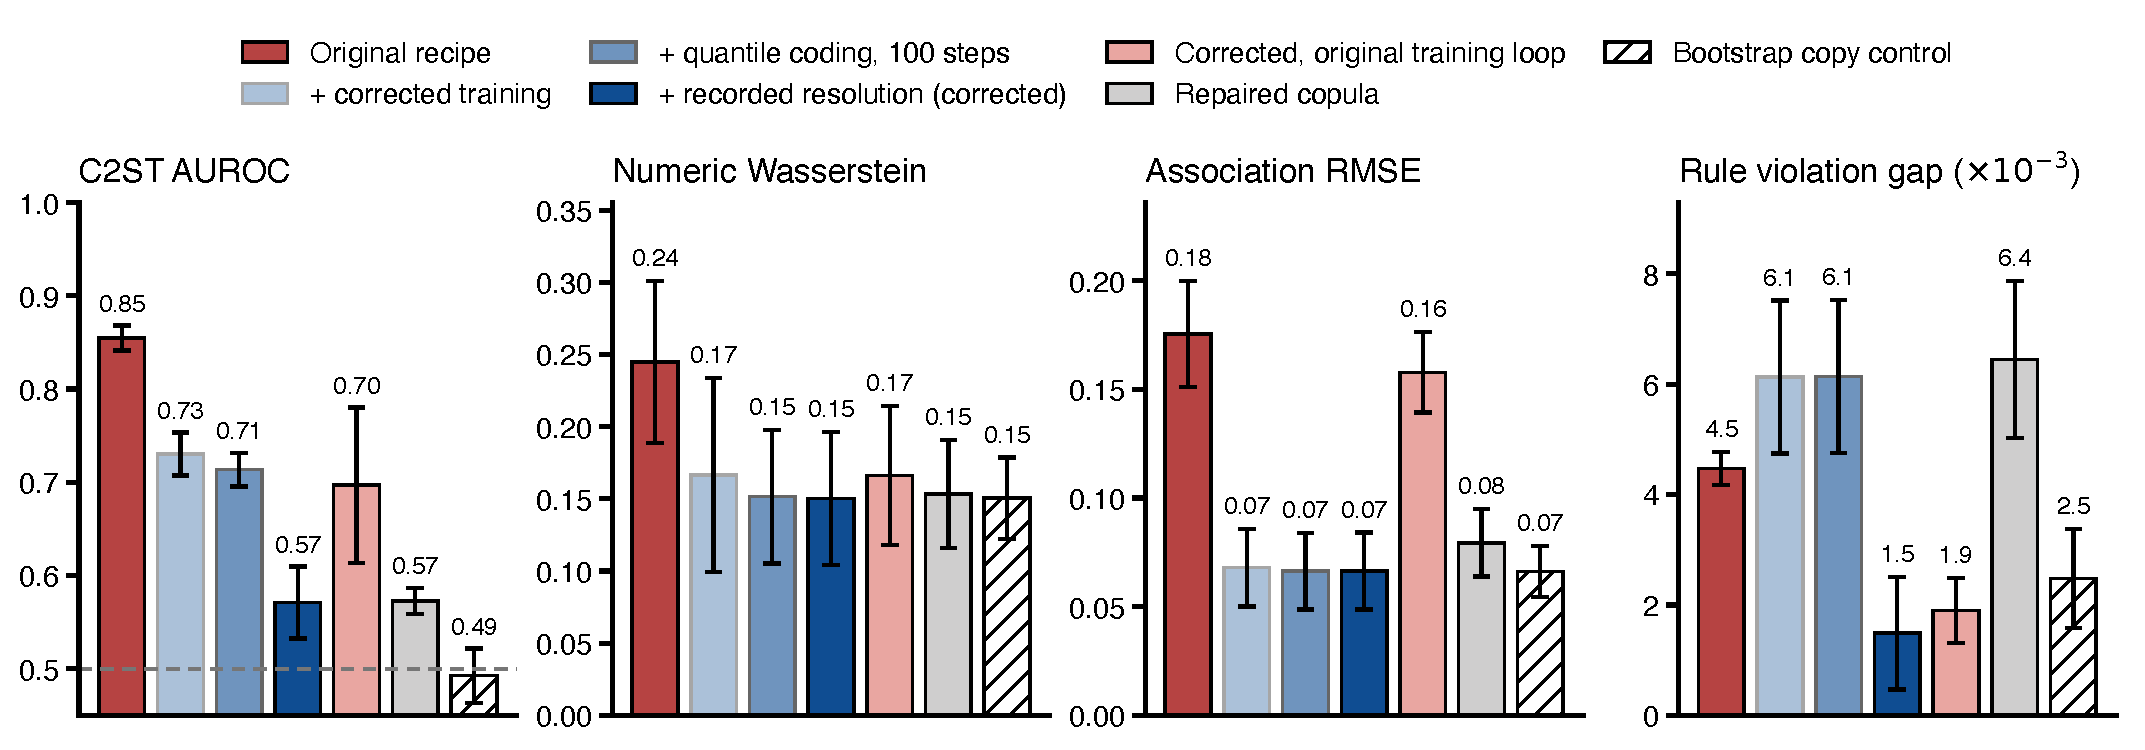
\includegraphics[width=\textwidth]{Figure2.pdf}
\caption{\textbf{Effect of each correction on the liver dataset development partitions.} Mean and standard deviation across three partitions. Blue shades accumulate the corrections; red bars are the original recipe and the corrected model with the original training loop; gray bars are references. Numeric Wasserstein is scaled by the training standard deviation and the rule gap is the difference between synthetic and real violation rates.}
\label{fig:ablation}
\end{figure}

\subsection*{Uncorrected versus corrected pipelines}

The uncorrected pipeline combines the choices of our development project: diffusion models trained with the legacy recipe, the adapter TabDDPM loop, raw outputs, two-sample tests on 100 records per source and no privacy check. We make no claim about how often these choices occur in published work. Compared with the corrected pipeline, it reversed the order of 25\% to 34\% of generator pairs and changed the top-ranked generator in 18 of 20 training samples (Table~\ref{tab:pipeline}, Fig.~\ref{fig:pipeline_rev}). The case-study model moved from the middle of the ranking to first place in 16 of 20 samples. A privacy-aware ranking, which places generators with membership AUROC above 0.60 last, changed by a similar amount.

\begin{table}[htbp]
\caption{Agreement between uncorrected and corrected pipelines for the realism ranking}
\label{tab:pipeline}
\centering
\footnotesize
\setlength{\tabcolsep}{3pt}
\begin{tabular}{lcccc}
\toprule
Population, $n$ & Pairs reversed & $\tau$ & Top-1 agree & Top (corrected) \\
\midrule
NHANES, 250 & 32\% (29 to 35) & 0.36 & 0/5 & MedHyperDiff \\
NHANES, 1000 & 34\% (29 to 38) & 0.33 & 0/5 & MedHyperDiff \\
Thyroid, 250 & 25\% (22 to 28) & 0.50 & 0/5 & MedHyperDiff \\
Thyroid, 1000 & 26\% (22 to 31) & 0.47 & 2/5 & MedHyperDiff \\
\bottomrule
\end{tabular}
\footnotetext{Pairs reversed: percentage of generator pairs whose order reverses, mean with 95\% bootstrap interval over five training samples in parentheses; $\tau$: Kendall's rank correlation; Top-1 agree: samples in which both pipelines rank the same generator first; Top (corrected): generator ranked first under the corrected pipeline.}
\end{table}

\begin{figure}[htbp]
\centering
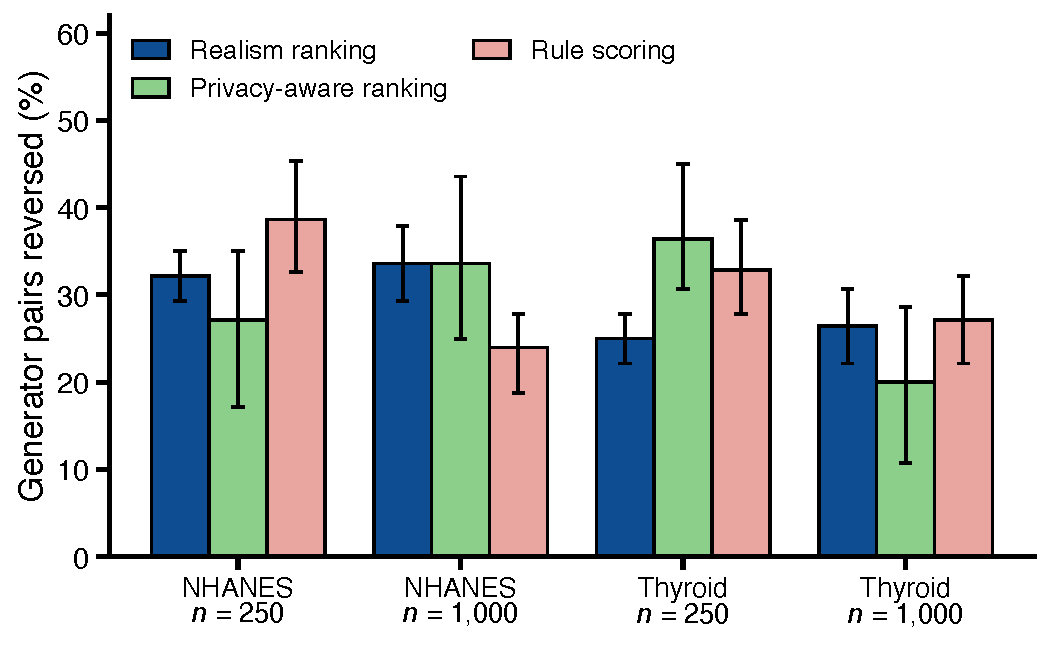
\includegraphics[width=85mm]{Figure3.pdf}
\caption{\textbf{Generator pairs whose order reverses between uncorrected and corrected pipelines.} Eight generator identities, for the realism ranking, the privacy-aware ranking and rule scoring (mean and 95\% bootstrap interval over five training samples).}
\label{fig:pipeline_rev}
\end{figure}

\subsection*{The training budget}

With the legacy recipe, 30\% of MedHyperDiff fits kept a checkpoint from the first 20 epochs and 45\% stopped at the epoch cap, and realism was worse than with the corrected recipe in all 20 training samples. The decomposition in Table~\ref{tab:decomp} identifies the cause. Giving the corrected recipe only the legacy number of updates reproduced the whole gap, whereas returning the validation-selected checkpoint, averaging the validation loss over corruption draws or stopping by patience had no consistent effect. The first pitfall is therefore an update budget that an epoch cap keeps too small on small tables, not validation-based selection itself. Two other training choices mattered: the earlier TabDDPM adapter loop diverged, and quantile coding of laboratory values helped in three of four settings but not in the fourth, so the numerical representation should be validated rather than assumed.

\begin{table}[htbp]
\caption{Decomposition of the training correction on the controlled-study samples}
\label{tab:decomp}
\centering
\footnotesize
\setlength{\tabcolsep}{2.4pt}
\begin{tabular}{lccccc}
\toprule
& \multicolumn{2}{c}{NHANES} & \multicolumn{2}{c}{Thyroid} & \\
Variant & 250 & 1000 & 250 & 1000 & Worse/better \\
\midrule
Corrected recipe & 0.729 & 0.691 & 0.710 & 0.686 & reference \\
+ validation-selected weights & 0.735 & 0.691 & 0.719 & 0.685 & 6/3 \\
+ selection with patience 20 & 0.778 & 0.691 & 0.710 & 0.685 & 5/6 \\
+ 16 corruption draws & 0.722 & 0.691 & 0.712 & 0.686 & 4/6 \\
Constant rate, raw weights & 0.786 & 0.689 & 0.754 & 0.683 & 13/7 \\
Legacy number of updates & 0.943 & 0.896 & 0.851 & 0.798 & 20/0 \\
Legacy, rebuilt & 0.945 & 0.832 & 0.862 & 0.760 & 20/0 \\
Legacy recipe & 0.951 & 0.857 & 0.866 & 0.756 & 20/0 \\
\bottomrule
\end{tabular}
\footnotetext{C2ST, mean of five samples per setting and nominal sample size. Worse/better: number of the 20 samples in which C2ST was worse or better than with the corrected recipe.}
\end{table}

\subsection*{Evaluation choices}

Decoding to the recorded resolution lowered the C2ST of MedHyperDiff by up to 0.31 and also improved TVAE, but hardly changed TabDDPM and TabDiff (Table~\ref{tab:precision}, Fig.~\ref{fig:precision}). The difference lies in the inverse transforms rather than the models: the quantile transforms of TabDDPM and TabDiff already return most values on the recording grid, which acts as an implicit decoding. Without explicit decoding, about 30\% of generator pairs on NHANES were ranked differently.

No learned generator reproduced the supplied relations: 90\% to 100\% of their NHANES records violated the globulin or body mass index identity, which no real record does, whereas re-deriving these variables reproduced real behavior. Scoring generators by violation counts instead of by the gap to real violation rates reordered some generator pairs but never changed the best generator.

Realism and memorization were linked. Across generators, a lower C2ST went with a higher membership AUROC (Fig.~\ref{fig:memo}), and the most realistic generator in a training sample exceeded a membership AUROC of 0.60 in up to 80\% of samples, depending on the setting. Realism metrics are therefore only interpretable alongside membership diagnostics.

Finally, small evaluation sets were unreliable. With the 60 to 120 test patients typical of public clinical cohorts, a single two-sample test ordered about one generator pair in six wrongly, and agreement with the full reference reached 90\% only at about 500 records per source (Table~\ref{tab:evalsize}, Fig.~\ref{fig:evalsize}).

\begin{table}[htbp]
\caption{C2ST by decoding at nominal sample size 1000}
\label{tab:precision}
\centering
\footnotesize
\setlength{\tabcolsep}{3pt}
\begin{tabular}{lccccc}
\toprule
& \multicolumn{2}{c}{NHANES} & \multicolumn{3}{c}{Thyroid} \\
Generator & Raw & Decoded & Raw & Global & Banded \\
\midrule
MedHyperDiff & 0.999 & 0.692 & 0.808 & 0.763 & 0.685 \\
TVAE & 0.991 & 0.913 & 0.950 & 0.947 & 0.934 \\
TabDiff & 0.703 & 0.703 & 0.698 & 0.696 & 0.692 \\
TabDDPM & 0.744 & 0.738 & 0.742 & 0.747 & 0.745 \\
\bottomrule
\end{tabular}
\footnotetext{Raw: continuous generator output; Decoded and Global: one recording grid per column detected on fit rows; Banded: grid per order of magnitude.}
\end{table}

\begin{figure}[htbp]
\centering
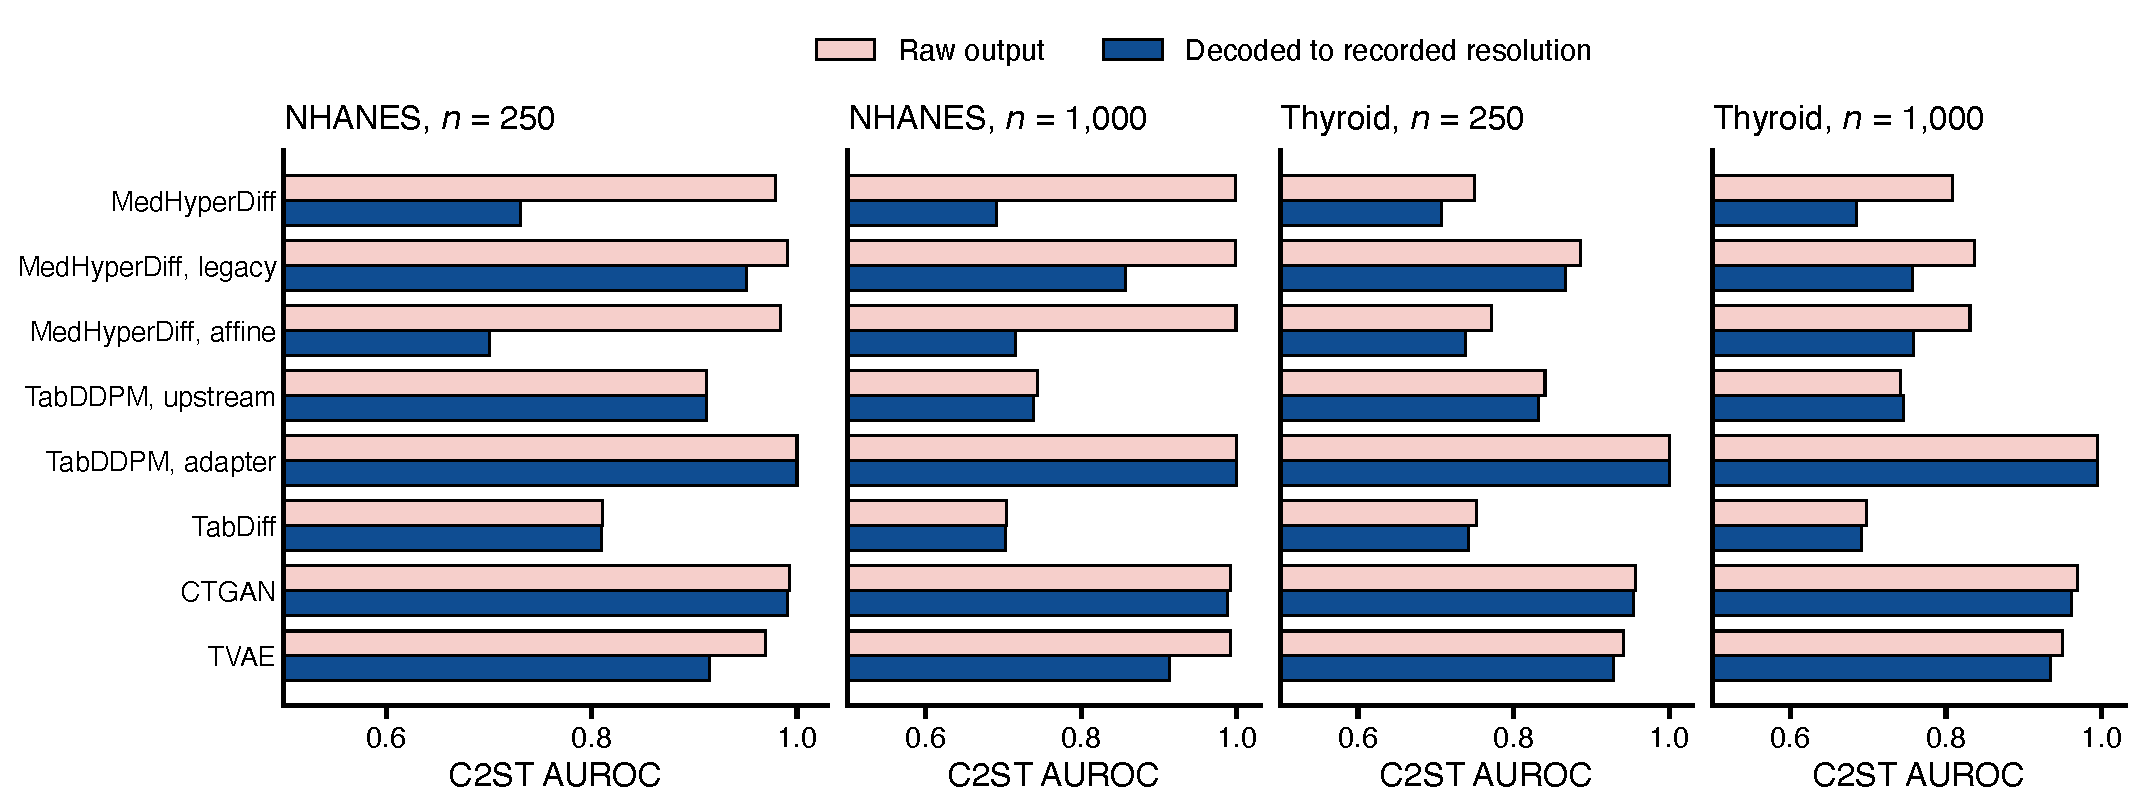
\includegraphics[width=\textwidth]{Figure4.pdf}
\caption{\textbf{C2ST of raw outputs and of outputs decoded to the recorded resolution.} Mean of five training samples; 0.5 is indistinguishable.}
\label{fig:precision}
\end{figure}

\begin{figure}[htbp]
\centering
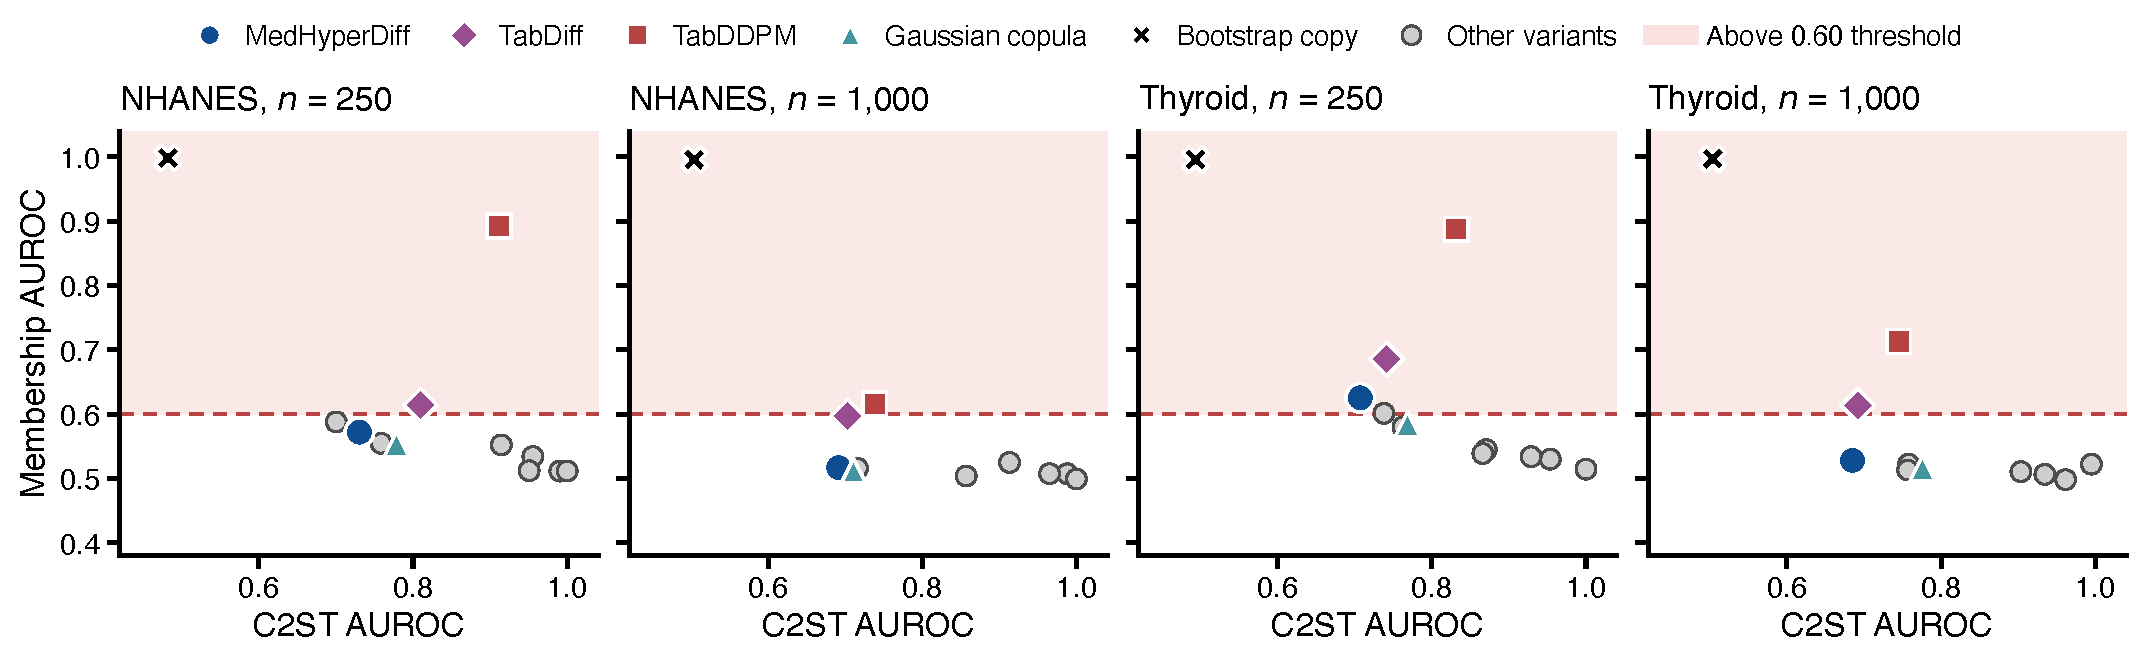
\includegraphics[width=\textwidth]{Figure5.pdf}
\caption{\textbf{Realism against membership risk for each generator.} Mean of five training samples. The shaded band marks a membership AUROC above 0.60 on at least one of two attacks.}
\label{fig:memo}
\end{figure}

\begin{table}[htbp]
\caption{Probability that one evaluation orders a generator pair correctly}
\label{tab:evalsize}
\centering
\footnotesize
\setlength{\tabcolsep}{4pt}
\begin{tabular}{lccccc}
\toprule
Records per source & 50 & 100 & 200 & 500 & 1000 \\
\midrule
NHANES & 0.77 & 0.85 & 0.88 & 0.93 & 0.96 \\
Thyroid & 0.78 & 0.84 & 0.90 & 0.94 & 0.95 \\
Pairs differing by at most 0.02 & 0.58 & 0.59 & 0.58 & 0.65 & 0.71 \\
Median single-draw SD & 0.062 & 0.045 & 0.031 & 0.015 & 0.008 \\
\bottomrule
\end{tabular}
\footnotetext{Probability that a single two-sample test on the given number of records per source orders a generator pair as the full reference does. SD: standard deviation of a single draw of the C2ST.}
\end{table}

\begin{figure}[htbp]
\centering
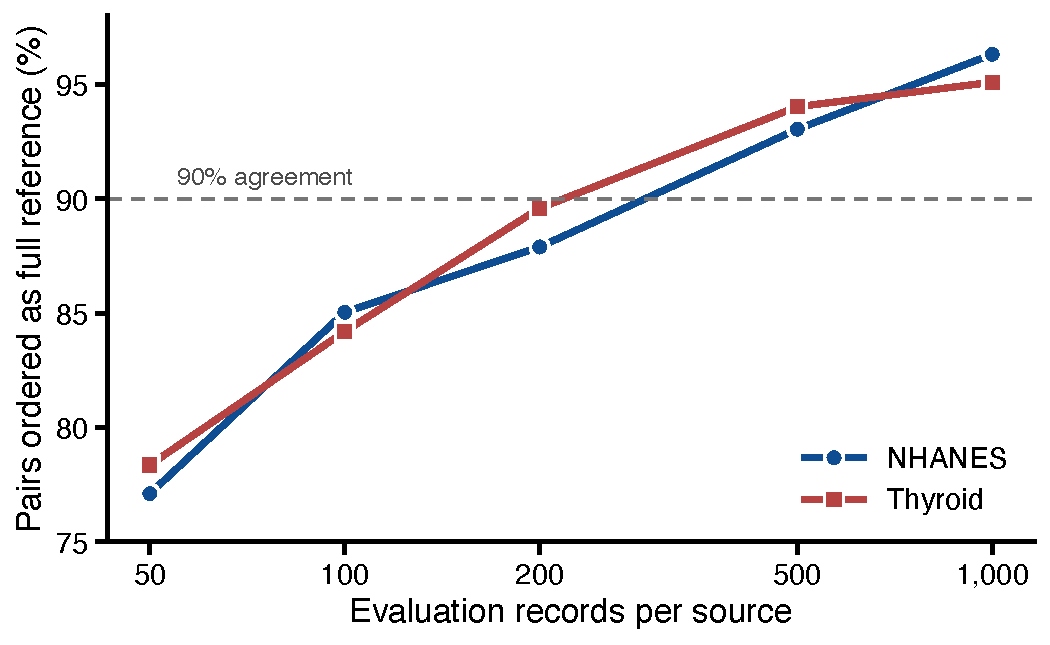
\includegraphics[width=85mm]{Figure6.pdf}
\caption{\textbf{Agreement between a single two-sample test and the full reference ordering.} Agreement as a function of evaluation size. The dashed line marks 90\%.}
\label{fig:evalsize}
\end{figure}

\subsection*{Relation fidelity}

The two kinds of laboratory relation behaved differently. For the approximate blood count relations, published generators as generated missed the relations by one to three orders of magnitude in relation distance, and deterministic re-derivation over-corrected them by removing the rounding discrepancies that real records have (Tables~\ref{tab:relation} and \ref{tab:robust}, Figs.~\ref{fig:relation} and \ref{fig:robust}). MedHyperDiff reproduced these relations most closely in all seven blood count settings, but controls that resample real residuals came close, so its advantage here is consistent rather than large. For the exact chemistry relations the order reversed: textbook re-derivation, which recomputes each derived value as the laboratory does, was the strongest control in four of five settings, and in every setting the strongest control was closer than our model. The direction of reconstruction also mattered. Recomputing narrow indices from generated operands, as textbook re-derivation does for blood counts, damaged realism and left a negative basophil fraction in 17\% of the rows of TabDiff on average, which supports choosing the reconstructed participant by Eq.~(\ref{eq:choice}).

Table~\ref{tab:diagnostics} shows what approximate relations require. Hematocrit, hemoglobin and red cell count enter three of the four blood count relations, so their residuals are correlated in real records. Methods that sample the residuals jointly, either by resampling the complete residual vector of a real record or by learning the residuals, preserved this coupling, whereas re-derivation and independent residual resampling, which treat each relation separately, roughly tripled the coupling error. Among the joint methods, the learned model reproduced the distribution of each residual more closely, while resampling kept the residuals more independent of other variables, as they are in real records. The benefit therefore comes from representing and sampling the residuals jointly rather than specifically from the hypergraph.

\begin{table}[htbp]
\caption{Relation fidelity, realism, utility and membership on the 2017 to 2018 blood counts}
\label{tab:relation}
\centering
\footnotesize
\setlength{\tabcolsep}{3pt}
\begin{tabular}{llcccc}
\toprule
$n$ & Measure & Ours & TabDiff & Best other arm & Wins \\
\midrule
\multirow{4}{*}{250} & Relation dist. & \textbf{0.187} & 12.14 & 0.199$^{a}$ & 3/5 \\
& C2ST & \textbf{0.691} & 0.762 & 0.731$^{b}$ & 5/5 \\
& TSTR AUROC & \textbf{0.717} & 0.670 & 0.687$^{c}$ & 5/5 \\
& Membership & 0.555 & 0.619 & 0.528$^{b}$ & \\
\midrule
\multirow{4}{*}{1000} & Relation dist. & \textbf{0.173} & 3.92 & 0.176$^{a}$ & 2/5 \\
& C2ST & 0.664 & 0.645 & \textbf{0.633}$^{d}$ & 0/5 \\
& TSTR AUROC & 0.735 & 0.735 & \textbf{0.742}$^{e}$ & 1/5 \\
& Membership & 0.509 & 0.560 & 0.561$^{d}$ & \\
\bottomrule
\end{tabular}
\footnotetext{Mean of five samples. Best other arm: lowest relation distance among all comparator arms, or lowest C2ST and highest TSTR AUROC among comparator arms with membership AUROC at most 0.60: $^{a}$TVAE with joint residuals, $^{b}$copula with rule-direction re-derivation, $^{c}$copula with independent residuals, $^{d}$TabDiff with rule-direction re-derivation, $^{e}$TabDiff with reparameterization. Wins: samples in which MedHyperDiff was better than that arm. Bold: best value.}
\end{table}

\begin{figure}[htbp]
\centering
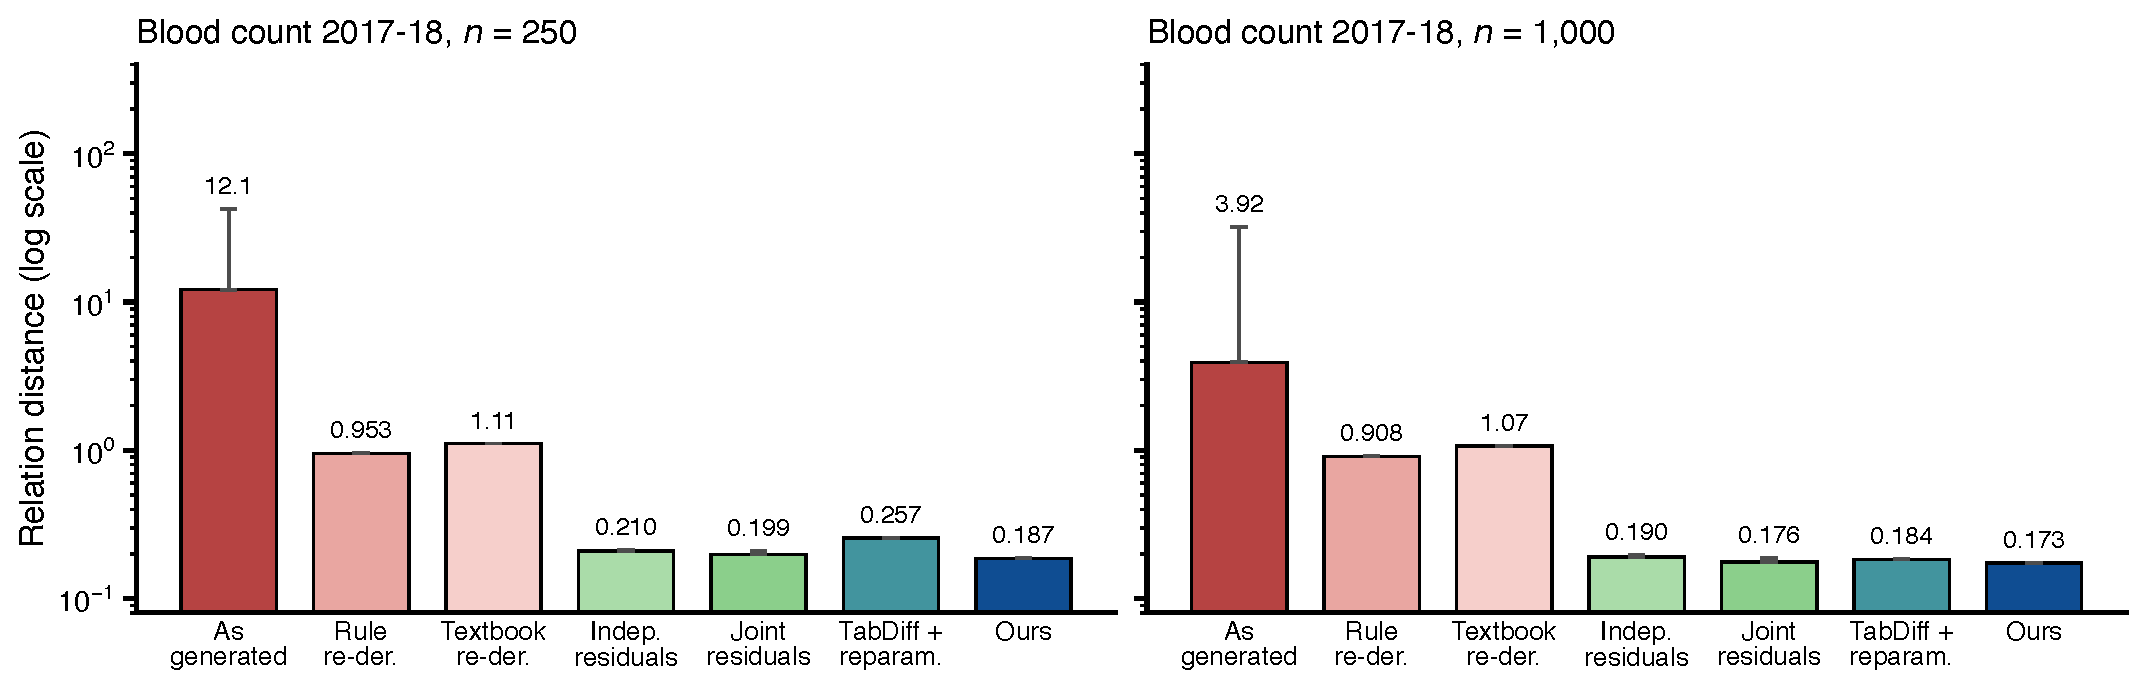
\includegraphics[width=\textwidth]{Figure7.pdf}
\caption{\textbf{Relation distance on the 2017 to 2018 blood counts.} Logarithmic scale. For each post-processing the bar shows the best of the five published generators and the whisker reaches their median. Rule and textbook re-der.: deterministic re-derivation in the reconstruction direction of our rule or in the textbook direction; indep. and joint residuals: real residuals resampled independently per relation or jointly per record; ours: MedHyperDiff with relation reparameterization.}
\label{fig:relation}
\end{figure}

\begin{table}[htbp]
\caption{Confirmation on four NHANES datasets by nominal sample size}
\label{tab:robust}
\centering
\footnotesize
\setlength{\tabcolsep}{2.2pt}
\begin{tabular}{llccccccccc}
\toprule
& & \multicolumn{3}{c}{Relation distance} & \multicolumn{3}{c}{C2ST} & \multicolumn{3}{c}{TSTR AUROC} \\
Dataset & $n$ & Ours & Control & Wins & Ours & Comparator & Wins & Ours & Comparator & Wins \\
\midrule
Blood count 2013-14 & 250 & \textbf{0.128} & 0.139 & 4/5 & \textbf{0.709} & 0.728 & 4/5 & \textbf{0.709} & 0.698 & 5/5 \\
 & 1000 & \textbf{0.092} & 0.106 & 5/5 & 0.646 & \textbf{0.634} & 1/5 & \textbf{0.771} & 0.753 & 5/5 \\
Blood count 2021-23 & 250 & \textbf{0.151} & 0.159 & 2/5 & \textbf{0.690} & 0.719 & 5/5 & \textbf{0.684} & 0.680 & 2/5 \\
 & 1000 & \textbf{0.137} & 0.156 & 4/5 & \textbf{0.629} & 0.634 & 2/5 & \textbf{0.733} & 0.723 & 4/5 \\
 & 2000 & \textbf{0.136} & 0.155 & 3/3 & 0.616 & \textbf{0.570} & 0/3 & 0.745 & 0.745 & 1/3 \\
Chemistry 2011-12 & 250 & 0.049 & \textbf{0.033} & 0/5 & 0.715$^{\dagger}$ & \textbf{0.737} & 4/5 & 0.878$^{\dagger}$ & \textbf{0.864} & 5/5 \\
 & 1000 & 0.025 & \textbf{0.019} & 2/5 & \textbf{0.644} & 0.674 & 5/5 & 0.888 & 0.888 & 3/5 \\
Chemistry 2021-23 & 250 & 0.050 & \textbf{0.027} & 0/5 & 0.775 & \textbf{0.760} & 1/5 & \textbf{0.895} & 0.882 & 5/5 \\
 & 1000 & 0.025 & \textbf{0.017} & 1/5 & \textbf{0.700} & 0.725 & 5/5 & 0.904 & \textbf{0.905} & 1/5 \\
 & 2000 & 0.021 & \textbf{0.015} & 1/3 & 0.645 & \textbf{0.620} & 0/3 & 0.905 & \textbf{0.907} & 1/3 \\
\bottomrule
\end{tabular}
\footnotetext{Mean over samples. Relation control: lowest relation distance among all comparator arms, that is published generators as generated, re-derived in either direction, with independently or jointly resampled residuals, or with reparameterization, chosen per setting in hindsight. Realism and utility comparators: the arm with the lowest C2ST or highest TSTR AUROC among comparator arms with mean membership AUROC at most 0.60. $\dagger$: MedHyperDiff exceeds that membership threshold. Bold: better value among eligible arms. Wins: samples in which MedHyperDiff was better.}
\end{table}

\begin{table}[htbp]
\caption{Relation diagnostics for residual-based and re-derived arms}
\label{tab:diagnostics}
\centering
\footnotesize
\setlength{\tabcolsep}{2pt}
\begin{tabular}{lcccccc}
\toprule
& \multicolumn{2}{c}{Relation dist.} & \multicolumn{2}{c}{Coupling} & \multicolumn{2}{c}{Dependence} \\
Arm & Blood & Chem. & Blood & Chem. & Blood & Chem. \\
\midrule
MedHyperDiff & \textbf{0.127} & 0.037 & 0.068 & \textbf{0.023} & 0.042 & 0.030 \\
TabDiff + reparam. & 0.168 & 0.051 & 0.069 & 0.025 & 0.043 & \textbf{0.028} \\
Copula, joint residuals & 0.152 & 0.046 & \textbf{0.061} & 0.025 & \textbf{0.029} & 0.030 \\
TabDiff, joint residuals & 0.155 & 0.047 & 0.062 & 0.024 & 0.031 & 0.030 \\
Copula, indep. residuals & 0.151 & 0.046 & 0.196 & 0.024 & 0.030 & 0.029 \\
TabDiff, re-der. (textbook) & 1.006 & \textbf{0.025} & 0.197 & \textbf{0.023} & 0.030 & 0.028 \\
TabDiff, re-der. (rule) & 0.867 & 0.327 & 0.202 & 0.024 & 0.031 & 0.029 \\
TabDiff, as generated & 10.56 & 4434 & 0.132 & 0.041 & 0.058 & 0.058 \\
\bottomrule
\end{tabular}
\footnotetext{Relation distance; error in the correlations between residuals of different relations (coupling); error in their correlations with participants, age and label (dependence). Mean over the two datasets of each panel and nominal sample sizes 250 and 1000; lower is better. Blood: blood count; Chem.: chemistry; re-der.: re-derivation in the reconstruction direction of our rule or in the textbook direction; indep.: independently resampled; reparam.: reparameterization. Bold: best value.}
\end{table}

\begin{figure}[htbp]
\centering
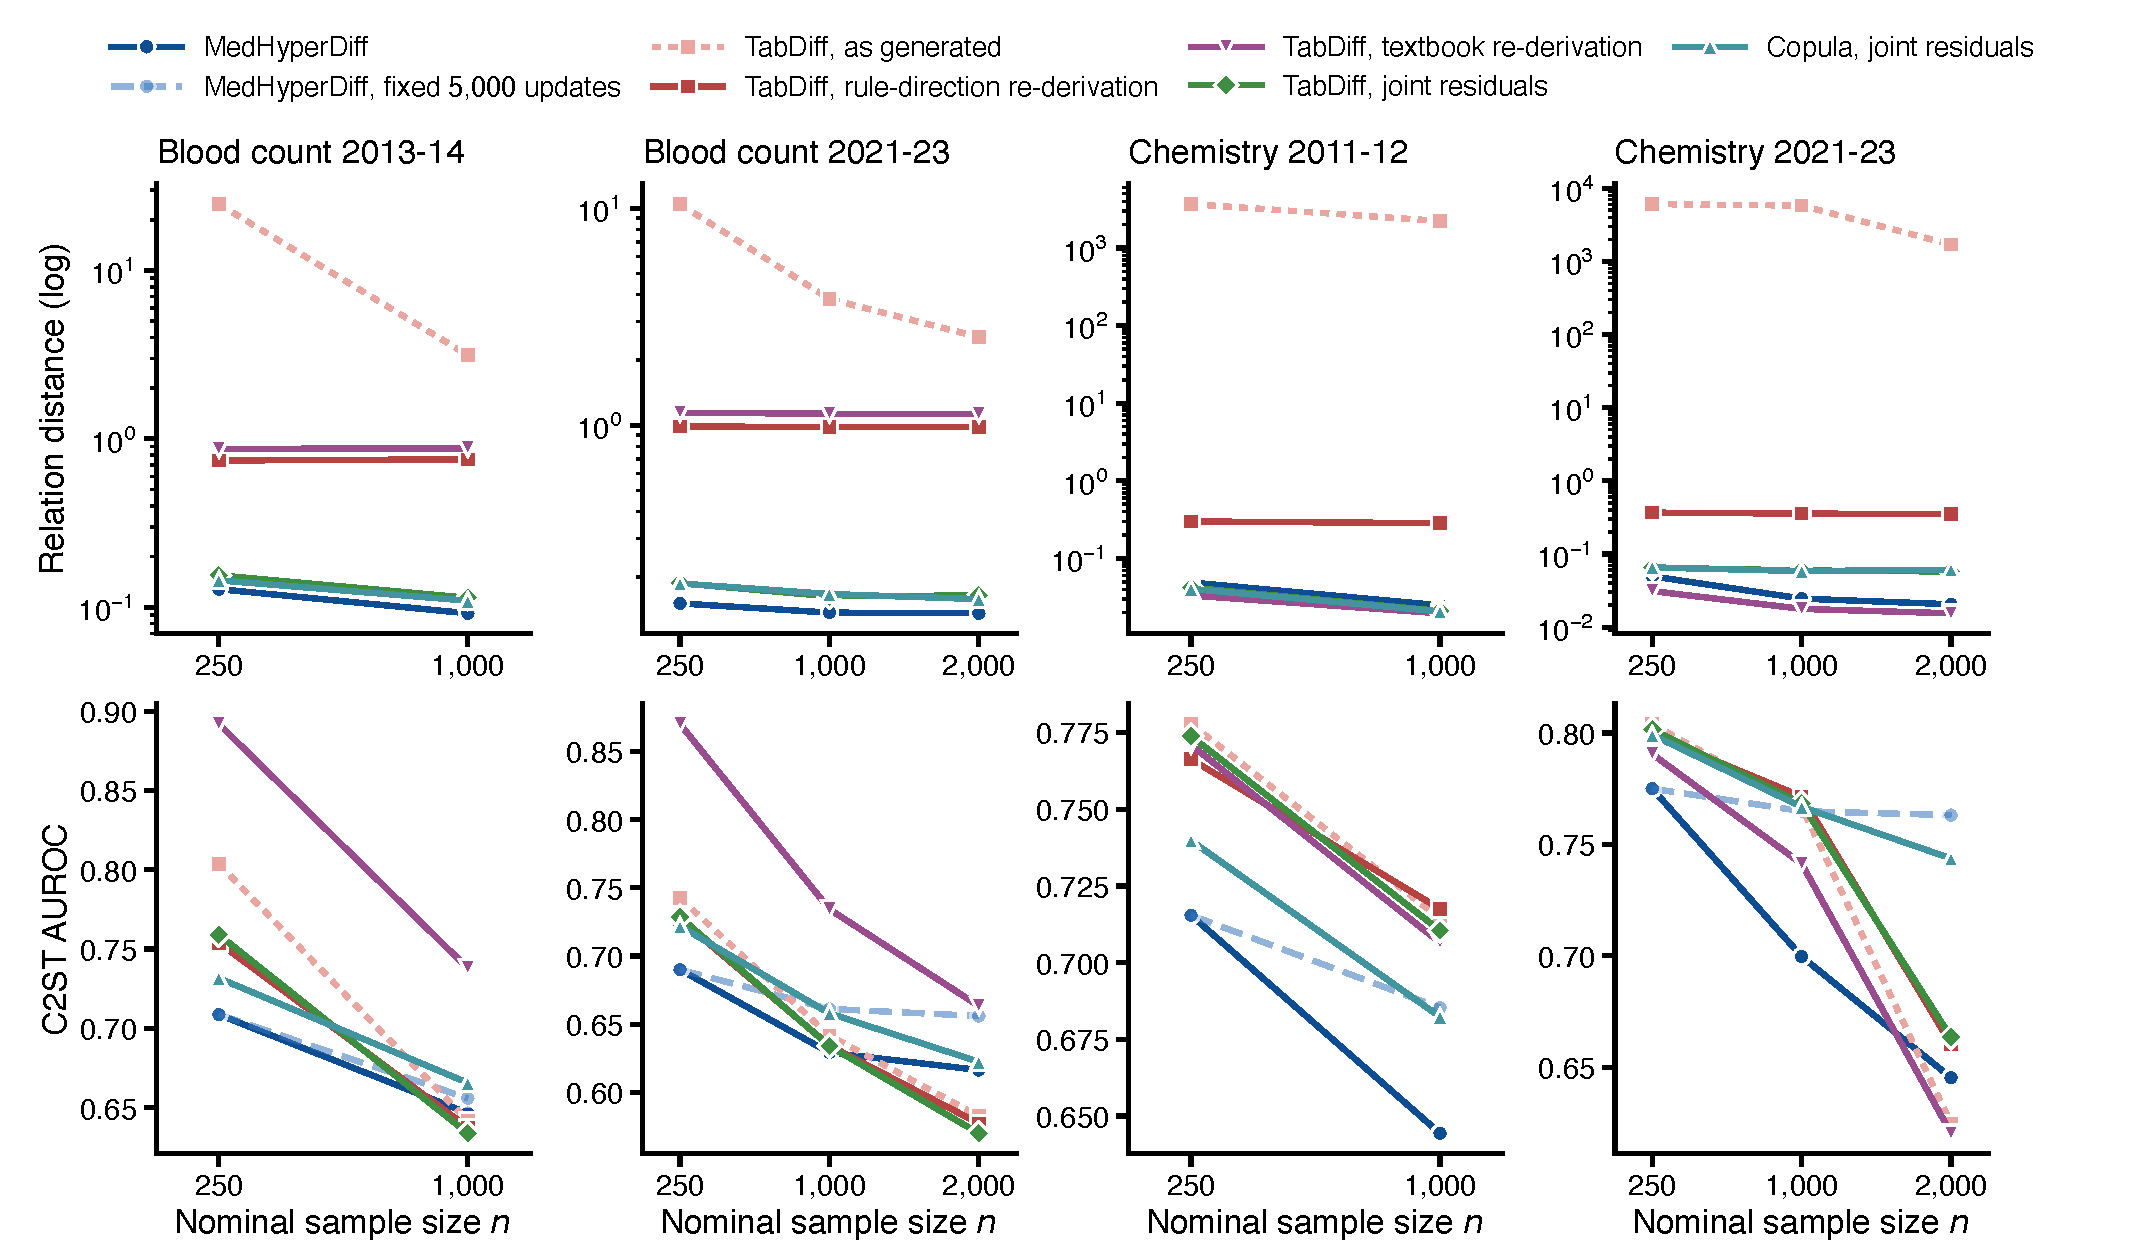
\includegraphics[width=\textwidth]{Figure8.pdf}
\caption{\textbf{Relation distance and C2ST on the four confirmation datasets by sample size.} Relation distance (top, logarithmic scale) and C2ST (bottom), mean over samples, by nominal sample size. Re-derivation is shown in the reconstruction direction of our rule and in the textbook direction; joint residuals are real residual vectors resampled after generation. The dashed line is MedHyperDiff with a fixed budget of 5000 updates.}
\label{fig:robust}
\end{figure}

\subsection*{Realism, utility and privacy}

With the membership threshold of 0.60 applied to every method, MedHyperDiff was the most realistic generator in five of ten settings, all at 250 or 1000 records (Table~\ref{tab:robust}). In the other five, TabDiff with joint residuals or a re-derivation control was more realistic, including in every sample at 2000 records, or the model itself exceeded the membership threshold. The advantages were small: averaged over the four datasets at 250 and 1000 records, the C2ST of the model was 0.012 to 0.014 lower than that of the best eligible comparator, and utility differed by about 0.01 in AUROC. Scaling the number of updates with the sample size was necessary for the model to keep improving with more data: with a fixed 5000 updates, as in the first relation test, realism stopped improving beyond 1000 records (Fig.~\ref{fig:robust}), and TabDiff with re-derivation was more realistic at that size (Table~\ref{tab:relation}). Better relation fidelity did not consistently translate into better agreement of relation-dependent clinical categories, mainly because re-derived and resampled controls already place most records in the correct categories.

The membership AUROC of the model stayed between 0.525 and 0.573 in nine of ten settings. At 100 records it rose to between 0.70 and 0.76, so the model should not be used on tables that small without stronger privacy protection. These attacks are diagnostics, and passing them does not establish that no patient can be identified.

\subsection*{Reparameterization as a plug-in and computation}

Added to TabDiff, TabDDPM and the copula, reparameterization lowered the relation distance of the raw output in every setting, but it is not a universal plug-in: the prespecified criterion that it should not raise C2ST by more than 0.02 held in 37 of 50 generator and setting combinations. CTGAN and TVAE generate implausible operands on the chemistry panel, such as urine creatinine near zero, which no post-processing can turn into a faithful ratio. MedHyperDiff has about 40 thousand parameters, against 10.8 million for TabDiff, and fitted in 5 to 42 minutes on a laptop central processing unit (CPU) (Table~\ref{tab:compute}), so its results did not come from a larger model or more computation. The comparison is nevertheless not tuning-matched, since the training budget of our model was selected on development data while the published generators used fixed configurations.

\begin{table}[htbp]
\caption{Computation of the diffusion models}
\label{tab:compute}
\centering
\footnotesize
\setlength{\tabcolsep}{2.5pt}
\begin{tabular}{lcccc}
\toprule
Model & Parameters & Updates & Passes & Minutes \\
\midrule
Ours & 39925 & 5k/20k/40k & 1600 & 5/20/42 \\
TabDiff & 10.8 M & 8k & 8000 & 36/95/157 \\
TabDDPM & 0.66 M & 30k & 30000 & 7/18/34 \\
\bottomrule
\end{tabular}
\footnotetext{Updates and median fit minutes at nominal sample sizes 250, 1000 and 2000, with eight concurrent single-threaded jobs on a laptop CPU. Passes: passes over the fit rows. k: thousand; M: million.}
\end{table}

\section*{Discussion}

The seven pitfalls change which generator appears best. Three of them, the training recipe, the numerical representation and baselines run outside their published recipes, change what the generators learn; the other four change only how the same outputs are scored. Together they reversed a quarter to a third of all comparisons in a controlled setting and most conclusions of a ten-iteration development project. The decomposition of the training correction also shows how a pitfall can be misattributed: the visible symptom was early checkpoints, but the main cause was the small number of updates that an epoch cap allows on small tables.

The relation studies separate three situations. For formulas computed exactly from reported values, recomputing the reported value from generated operands in the textbook direction was the most faithful choice and should be standard practice for any generator. For approximate formulas, exact enforcement and independent residual noise are both wrong: the first removes discrepancies that real records have, and the second breaks the coupling between formulas that share participants. Sampling the residuals jointly, whether by resampling real residual vectors or by learning them, preserves that coupling; the learned model reproduced each residual distribution somewhat more closely, while resampling kept residuals independent of other variables. The direction of reconstruction matters as well: recomputing narrow indices from generated operands degraded realism and produced negative basophil fractions.

Beyond relations, the proposed model was the most realistic generator below the membership threshold in five of ten settings, all at 250 or 1000 records, with a small utility advantage and about 40 thousand parameters; TabDiff or simple controls were as realistic or more in the other settings and at 2000 records. Small datasets with known laboratory relations are common, since rare diseases, single-site cohorts, pediatric studies and most public clinical tables contain hundreds rather than thousands of patients. The hypergraph itself was not isolated: TabDiff with the same reparameterization and joint residual resampling reached similar coupling, so the evidence supports the residual representation and joint sampling rather than the architecture. A matched ablation of the final model with and without graph and hypergraph, tuned baselines and untouched data are the most direct next tests, and evaluation on hospital data from another source would be needed for claims beyond NHANES.

\subsection*{A corrected protocol}

The results suggest a corrected protocol with seven elements. Diffusion models should be trained with an optimization budget chosen during development and scaled with the training size rather than capped in epochs, with learning-rate decay and weight averaging, and any validation-based selection should report the selected updates. The numerical representation should be validated rather than assumed. Every continuous-output generator should be decoded to the recorded resolution, per order of magnitude where reporting uses significant figures, and the on-grid fraction of raw outputs should be reported. Relations computed exactly should be re-derived in the direction the laboratory computes them; approximate relations should keep their residuals, sampled jointly across relations that share participants, and should be scored against real held-out behavior through signed and absolute residual distances and coupling and dependence diagnostics. Baselines should be run with their upstream training loops, and generators that use relation knowledge should be compared with simple post-processing controls that use the same knowledge. Membership diagnostics with at least a nearest-distance attack, a density-ratio attack and a copy control should accompany every realism metric, and the same membership threshold should apply to every method, including the proposed one. In our setting, two-sample tests needed about 500 records per source to order pairs reliably, and differences below 0.02 were often unresolved.

\subsection*{Limitations}

All relation datasets come from NHANES, analyzed without survey weights, and several share participants across panels; results may not transfer to hospital records, other laboratories, longitudinal data or other missingness mechanisms. Comparators used fixed configurations while our training budget was selected on development data. Textbook re-derivation and joint residual resampling were added after the confirmation outputs had been examined, and joint resampling ignores any dependence of residuals on other variables. Results at $n = 2000$ rest on three heavily overlapping samples in two datasets, the 100-record condition was removed by amendment, and differences are conditional on fixed reference halves. The primary relation metric uses absolute residuals, and the diagnostics that address sign and dependence were added after the confirmation. Utility was measured for a single prediction task with one model, and no intended clinical use was evaluated directly. Membership attacks are empirical diagnostics, the threshold of 0.60 is a convention, and no formal privacy guarantee is claimed. The protocols were dated and hashed locally rather than registered publicly. TabDDPM and TabDiff are adaptations of pinned upstream code rather than reproductions of their published benchmarks.

\section*{Conclusions}

Routine training and evaluation choices can determine which synthetic data generator appears best on small clinical tables, reversing a quarter to a third of comparisons in a controlled study, and damage attributed to checkpoint selection came mainly from an epoch-capped update budget. Laboratory relations need different treatments: formulas computed exactly from reported values are best recomputed, whereas approximate formulas need residuals that are kept and sampled jointly. A diffusion model with learned residual coding reproduced the approximate blood count relations most closely in every setting across three survey cycles, by a small margin over joint residual resampling, and was the most realistic generator below a prespecified membership threshold in five of ten settings, all at 250 or 1000 records; simple controls or TabDiff matched or exceeded it elsewhere, including at 2000 records. Future work should isolate the contribution of the hypergraph with a matched ablation, compare tuned baselines on untouched data with participant-consistent splits, apply stronger membership attacks, and evaluate hospital data from other laboratories and an intended clinical use.

\backmatter

\section*{List of abbreviations}

\begin{tabular}{@{}lp{0.8\textwidth}@{}}
AUROC & Area under the receiver operating characteristic curve \\
BMI & Body mass index \\
BUN & Blood urea nitrogen \\
C2ST & Classifier two-sample test \\
CPU & Central processing unit \\
CTGAN & Conditional tabular generative adversarial network \\
DOMIAS & Detecting overfitting for membership inference attacks on synthetic data \\
Hct & Hematocrit \\
MCV & Mean corpuscular volume \\
NHANES & National Health and Nutrition Examination Survey \\
RBC & Red blood cell count \\
SD & Standard deviation \\
TabDDPM & Tabular denoising diffusion probabilistic model \\
TSTR & Train on synthetic, test on real \\
TVAE & Tabular variational autoencoder \\
UCI & University of California, Irvine \\
\end{tabular}

\section*{Declarations}

\subsection*{Ethics approval and consent to participate}
This study is a secondary analysis of publicly available, de-identified data; no new data were collected and no participants were contacted. The NHANES protocols were approved by the Ethics Review Board of the National Center for Health Statistics (Protocol \#2011-17 and its continuations for 2011 to 2016, Protocol \#2018-01 for 2017 to 2018 and Protocol \#2021-05 for 2021 to 2023) \cite{nhaneserb}, and NHANES participants provide informed consent before taking part. The UCI datasets were obtained from the UCI Machine Learning Repository as released by their contributors.

\subsection*{Consent for publication}
Not applicable.

\subsection*{Availability of data and materials}
The datasets analysed during the current study are publicly available: the NHANES public-use files from the National Center for Health Statistics \cite{nhanes2011,nhanes2013,nhanes2015,nhanes2017,nhanes2021} and the UCI Machine Learning Repository datasets \cite{ilpd,heartfailure,ckd,diabetes,thyroid}, which are cited with their persistent identifiers. NHANES public-use data may be used only for statistical reporting and analysis, and any attempt to identify a participant is prohibited. The source code, the experiment and analysis scripts, the study protocols and the aggregated results underlying every table and figure, as comma-separated values files, are available in the MedHyperDiff repository \cite{code}. The repository contains scripts that download the public source files; no participant-level records are redistributed.

Project name: MedHyperDiff. Project home page: \url{https://github.com/NarenTheNumpkin/MHD}. Operating system: platform independent (tested on macOS). Programming language: Python. Other requirements: Python 3.11 to 3.13, PyTorch 2.14 and the pinned dependencies listed in the repository. License: MIT. Any restrictions to use by non-academics: none.

\subsection*{Competing interests}
The authors declare that they have no competing interests.

\subsection*{Funding}
This research received no specific grant from any funding agency in the public, commercial or not-for-profit sectors.

\subsection*{Authors' contributions}
NM was the principal investigator and main contributor, and conceived and designed the study, developed the software, ran the experiments, analysed and interpreted the results, and wrote the manuscript. AKG and RP assisted with the experiments, the analysis and the revision of the manuscript. PK oversaw the project and provided guidance on the study design, the interpretation of the results and the manuscript. All authors read and approved the final manuscript.

\subsection*{Acknowledgements}
We thank the National Center for Health Statistics for NHANES, the Garvan Institute and Ross Quinlan for the thyroid data, and the UCI Machine Learning Repository.

\bibliography{references}

\end{document}
